%==============================================================================
% CONFIGURAÇÃO DO DOCUMENTO
%==============================================================================
\documentclass[a4paper,12pt]{extarticle}  % Classe de documento com tamanho A4 e fonte 12pt

%==============================================================================
% PACOTES E BIBLIOTECAS
%==============================================================================

% --- Configuração de página e layout ---
\usepackage[left=30mm,top=30mm,right=30mm,bottom=30mm]{geometry}  % Margens do documento
\usepackage{etoolbox}     % Necessário para a página de capa
\usepackage{adjustbox}    % Ajustes de caixas
\usepackage{fancyhdr}     % Cabeçalho e rodapé personalizados
\setlength{\headheight}{15.05pt} % Corrige erro do fancyhdr sobre headheight
\usepackage{lastpage}     % Referência à última página

% --- Suporte a idiomas e codificação ---
\usepackage[T1]{fontenc}  % Codificação de fontes
\usepackage[utf8]{inputenc}  % Suporte a caracteres UTF-8
\usepackage[portuguese]{babel}  % Suporte ao idioma português
\usepackage{newunicodechar}
\newunicodechar{₋}{$_-$}

% --- Matemática e símbolos ---
\usepackage{amsmath}      % Funções matemáticas avançadas
\usepackage{amsfonts}     % Fontes matemáticas adicionais
\usepackage{mathtools}    % Extensões para o amsmath
\usepackage{amssymb}      % Símbolos matemáticos adicionais
\usepackage{bm}           % Símbolos matemáticos em negrito
\usepackage{siunitx}      % Formatação de unidades do SI

% --- Figuras e elementos visuais ---
\usepackage{graphicx}     % Inclusão de figuras
\usepackage{subcaption}   % Suporte a subfiguras
\usepackage[table]{xcolor} % Suporte a cores e cores em tabelas
\usepackage{float}        % Melhor controle do posicionamento de figuras
\usepackage{tikz}         % Criação de diagramas
\usetikzlibrary{shapes.geometric, arrows}

% --- Tabelas e listas ---
\usepackage{booktabs}     % Melhora a aparência das tabelas
\usepackage{multirow}     % Células que ocupam múltiplas linhas
\usepackage{enumitem,kantlipsum}  % Personalização de listas
\usepackage[usestackEOL]{stackengine}  % Manipulação de texto em pilha

% --- Algoritmos e código ---
\usepackage[ruled,vlined]{algorithm2e}  % Algoritmos em pseudocódigo
\usepackage{listings}     % Inclusão de código-fonte
\usepackage{minted}       % Destaque de sintaxe avançado
\usemintedstyle{emacs}    % Estilo de cores para código
\usepackage{tcolorbox}    % Caixas coloridas para código/exemplos

% --- Títulos e formatação de seções ---
\usepackage{titlesec}     % Personalização de títulos de seções
\usepackage{titletoc}     % Personalização do sumário

% --- Referências e links ---
\usepackage[square,numbers,sort]{natbib}  % Gerenciamento de bibliografia
\usepackage{hyperref}     % Hiperlinks no documento
\usepackage[capitalise]{cleveref}  % Referências cruzadas inteligentes

%==============================================================================
% CONFIGURAÇÕES PERSONALIZADAS
%==============================================================================

% --- Configuração de blocos de exemplo ---
\newtcolorbox[auto counter, number within=section]{exampleblock}[2][]{
    colframe=gray!80!black, 
    colback=white, 
    coltitle=black, 
    title=Exemplo \thetcbcounter: #2, 
    #1, 
    fonttitle=\bfseries, 
    sharp corners=southwest
}

% --- Definição de cores ---
\definecolor{azulTitulos}{RGB}{0, 76, 153}  % Define uma cor azul para títulos

% --- Formatação de títulos de seções ---
\titleformat{\section}
  {\color{azulTitulos}\normalfont\Large\bfseries}  % Seções em azul, grande e negrito
  {\thesection}{1em}{}
\titleformat{\subsection}
  {\color{azulTitulos}\normalfont\large\bfseries}  % Subseções em azul, menor e negrito
  {\thesubsection}{1em}{}

% --- Configuração de hiperlinks ---
\hypersetup{
    colorlinks,  % Ativa links coloridos
    linkcolor={black},  % Links internos em preto
    citecolor={blue!50!black},  % Citações em azul escuro
    urlcolor={blue!80!black}  % URLs em azul mais claro
}

% --- Configuração do cabeçalho e rodapé ---
\pagestyle{fancy}
\fancyhf{}
\fancyhead[L]{\leftmark}
\fancyhead[R]{\thepage}
\fancyfoot[L]{CSR}
\fancyfoot[C]{Laboratório 1}
\fancyfoot[R]{\thepage\ de \pageref{LastPage}}
\renewcommand{\headrulewidth}{0.4pt}
\renewcommand{\footrulewidth}{0.4pt}

% --- Estilos de página especiais ---
% Estilo para páginas de capítulo e primeira página
\fancypagestyle{plain}{
    \fancyhf{}
    \fancyfoot[C]{Título do Documento}
    \fancyfoot[R]{Página \thepage\ de \pageref{LastPage}}
    \renewcommand{\headrulewidth}{0pt}
    \renewcommand{\footrulewidth}{0.4pt}
}

% Estilo para primeira página (sem cabeçalho nem rodapé)
\fancypagestyle{firstpage}{
    \fancyhf{}
    \renewcommand{\headrulewidth}{0pt}
    \renewcommand{\footrulewidth}{0pt}
}

% --- Configurações gerais ---
\linespread{1}  % Espaçamento de linha simples
\newtheorem{theorem}{Theorem}[section]  % Define ambiente para teoremas
\graphicspath{{img/}}  % Pasta para figuras

% --- Listings settings ---
\lstset{
  language=Python,
  basicstyle=\ttfamily\footnotesize,
  keywordstyle=\color{blue}\bfseries,
  stringstyle=\color{red},
  commentstyle=\color{gray}\itshape,
  numbers=left,
  numberstyle=\tiny\color{gray},
  stepnumber=1,
  numbersep=8pt,
  backgroundcolor=\color{white},
  showspaces=false,
  showstringspaces=false,
  showtabs=false,
  frame=single,
  rulecolor=\color{black},
  tabsize=4,
  captionpos=b,
  breaklines=true,
  breakatwhitespace=true,
  morekeywords={self},
}


%==============================================================================
% CORPO DO DOCUMENTO
%==============================================================================
\begin{document}

%==============================================================================
% PÁGINAS PRÉ-TEXTUAIS
%==============================================================================
% --- Página de capa ---
\pagenumbering{gobble}  % Remove a numeração de páginas inicialmente
\thispagestyle{firstpage}
\newcommand{\bonecoUM}{Aniko Costa}          % Nome do primeiro docente
\newcommand{\bonecoDOIS}{Filipe Moutinho}        % Nome do segundo docente
\newcommand{\docenteTRES}{}                    % Espaço para um terceiro docente (vazio)
\newcommand{\alunoUM}{João Pedro Antunes - \textbf{70380}}      % Nome e número do terceiro aluno
\newcommand{\alunoDOIS}{Júlio Lopes- \textbf{70512}}  % Nome e número do segundo aluno
\newcommand{\judeu}{Marco Romao - \textbf{71348}}      % Nome e número do terceiro aluno
\newcommand{\data}{1º Semestre 2025/2026}      % Período académico 
\newcommand{\cadeira}{Co-design e Sistemas Reconfiguráveis}  % cadeira
\newcommand{\titulo}{Laboratório 1}       % Título do trabalho 
\title{Título} %n mudar                        % Título alternativo (não usado na capa)
\newcommand{\departmento}{Departamento de Engenharia Eletrotécnica e de Computadores}  % Nome do departamento
\newcommand{\curso}{Mestrado em Engenharia Eletrotécnica e de Computadores}  % Nome do curso
% -------------------------------- Front content
\begin{center}\leavevmode                      % Inicia o ambiente centralizado da capa
    \normalfont
    
\includegraphics[width=0.75\columnwidth]{img/logo.png}  % Logotipo da instituição
    \vskip 1cm                                 % Espaçamento vertical de 1cm
    \textsc{\Large \departmento}\\[1 cm]       % Nome do departamento em maiúsculas pequenas
    {\large \curso}                            % Nome do curso
    \vskip 1cm                                 % Espaçamento vertical de 1cm
    \rule{\linewidth}{0.2 mm}                  % Linha horizontal decorativa
    {\huge \bfseries \titulo \par}             % Título em negrito e tamanho enorme
    \vskip 1cm                                 % Espaçamento vertical de 1cm
    {\Large \bfseries \cadeira \par}          % Subtítulo em negrito e tamanho grande
           
    \rule{\linewidth}{0.2 mm}\\[1.5 cm]        % Linha horizontal decorativa com espaçamento
     
    \begin{minipage}[t]{0.45\textwidth}        % Coluna esquerda para informações dos alunos
    	\begin{flushleft} \large
    		\emph{Alunos:}\\
    		\ifdefempty{\alunoUM}{}{\alunoUM\\}     % Verifica e exibe o aluno 1 se definido
            \ifdefempty{\alunoDOIS}{}{\alunoDOIS\\} % Verifica e exibe o aluno 2 se definido
            \ifdefempty{\judeu}{}{\judeu\\}         % Verifica e exibe o aluno 3 se definido
    	\end{flushleft}
    \end{minipage}
    \begin{minipage}[t]{0.45\textwidth}        % Coluna direita para informações dos docentes
        \begin{flushright} \large
        	{\emph{Docentes:}}\\
        	\ifdefempty{\bonecoUM}{}{\bonecoUM\\}       % Verifica e exibe o docente 1 se definido
        	\ifdefempty{\bonecoDOIS}{}{\bonecoDOIS\\}   % Verifica e exibe o docente 2 se definido
        	\ifdefempty{\docenteTRES}{}{\docenteTRES\\} % Verifica e exibe o docente 3 se definido
        \end{flushright}
    \end{minipage}
    \vfill                                     % Preenche o espaço vertical restante
    {\normalsize \data\par}                    % Data do semestre acadêmico
\end{center}
\cleardoublepage                               % Finaliza a página e inicia uma nova página (ímpar)  % Inclui a página de capa

% --- Sumário e listas ---
\newpage
\pagenumbering{roman}
\setcounter{page}{1}

\tableofcontents
\newpage

% Listas opcionais (comentadas)
%\listoffigures
%\newpage
%\listoftables
%\newpage
%\listofalgorithms  % Lista de algoritmos em pseudocódigo
%\newpage
%\listoflistings  % Lista de algoritmos em formato de código
%\newpage

%==============================================================================
% CONTEÚDO PRINCIPAL
%==============================================================================
\pagenumbering{arabic}  % Inicia numeração arábica (1, 2, 3...)
\setcounter{page}{1}

% --- Seções do documento ---
\section{Introdução}

\subsection{Contextualização}
%Contextualização do problema (sistema de automação com N células em cascata)

Este trabalho insere-se no âmbito da unidade curricular de Co-design e Sistemas Reconfiguráveis, focando-se no desenvolvimento e implementação de controladores para sistemas de automação industrial. O caso de estudo considerado é um sistema de produção composto por 3 células em cascata, onde cada célula integra um braço de robô e um tapete rolante.

A complexidade destes sistemas justifica a utilização de metodologias formais de modelação e verificação, permitindo validar o comportamento do controlador antes da sua implementação física. Adicionalmente, a possibilidade de implementar o controlador de forma centralizada ou distribuída oferece diferentes trade-offs entre complexidade de implementação, desempenho e escalabilidade do sistema.

\subsection{Objetivos}
%Objetivos do trabalho
O presente trabalho tem como objetivo principal o desenvolvimento completo de um controlador para um sistema de automação com três células em cascata (N=3), desde a fase de modelação até à implementação física em hardware reconfigurável.

Os objetivos específicos incluem:

\begin{itemize}
    \item Modelar o comportamento do sistema utilizando redes de Petri Input-Output Place-Transition (IOPT), explorando as capacidades de composição modular através de operações de adição e fusão de redes;
    
    \item Validar e analisar o modelo através de simulação e análise do espaço de estados, verificando propriedades comportamentais críticas do sistema;
    
    \item Implementar o controlador em plataformas de hardware distintas (FPGA e Arduino), avaliando a abordagem centralizada de controlo;
    
    \item Desenvolver uma arquitetura de controlo distribuído através da decomposição do modelo global, explorando paradigmas de execução síncrona e GALS (Globally Asynchronous Locally Synchronous);
    
    \item Analisar o impacto de comunicações não-instantâneas entre controladores distribuídos, introduzindo atrasos pseudo-aleatórios;
    
    \item Estender o modelo para suportar buffers de capacidade finita superior a uma unidade, aumentando a flexibilidade do sistema;
    
    \item Comparar as diferentes abordagens de implementação, avaliando vantagens, desvantagens e adequação a diferentes contextos aplicacionais.
\end{itemize}
\clearpage

\section{Análise Teórica}

\subsection{Redes de Petri}
%Redes de Petri e Redes de Petri Coloridas

\subsection{Execução síncrona vs. GALS}
%Paradigma de execução síncrona vs. GALS (Globally Asynchronous Locally Synchronous)

\subsection{Implementação em FPGA e Arduino}
%Conceitos de implementação em FPGA e Arduino


\clearpage

\section{Redes de Petri}

\subsection{IOPT-Tools}

\subsubsection{Rede de Petri - Tapete Singular}
\begin{figure}[H]
    \centering
    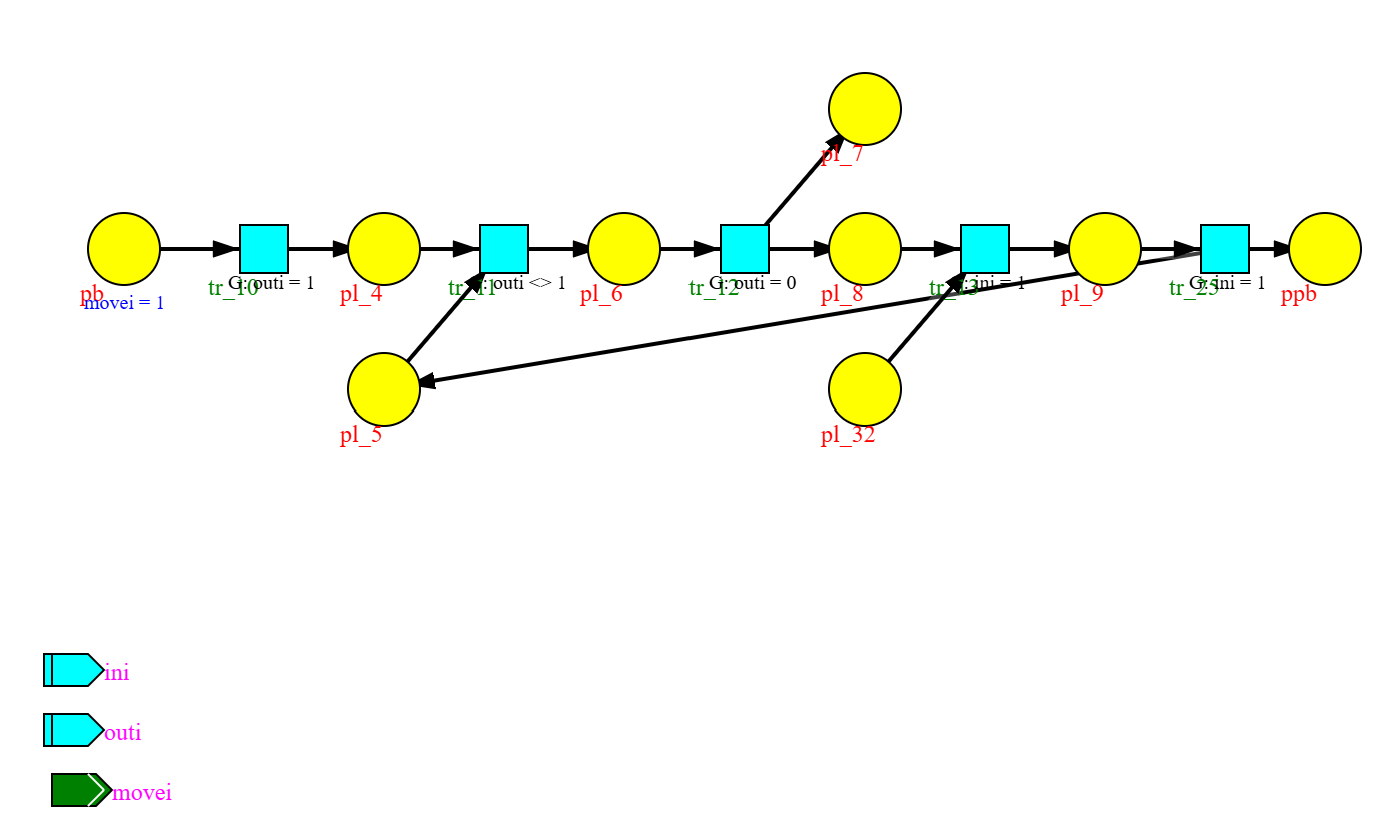
\includegraphics[width=0.8\textwidth]{img/petri_tapete_singular.png}
    \caption{Rede de Petri - Tapete Singular}
    \label{fig:petri_tapete_singular}
\end{figure}

\subsubsection{Rede de Petri - Modelo Completo}
\begin{figure}[H]
    \centering
    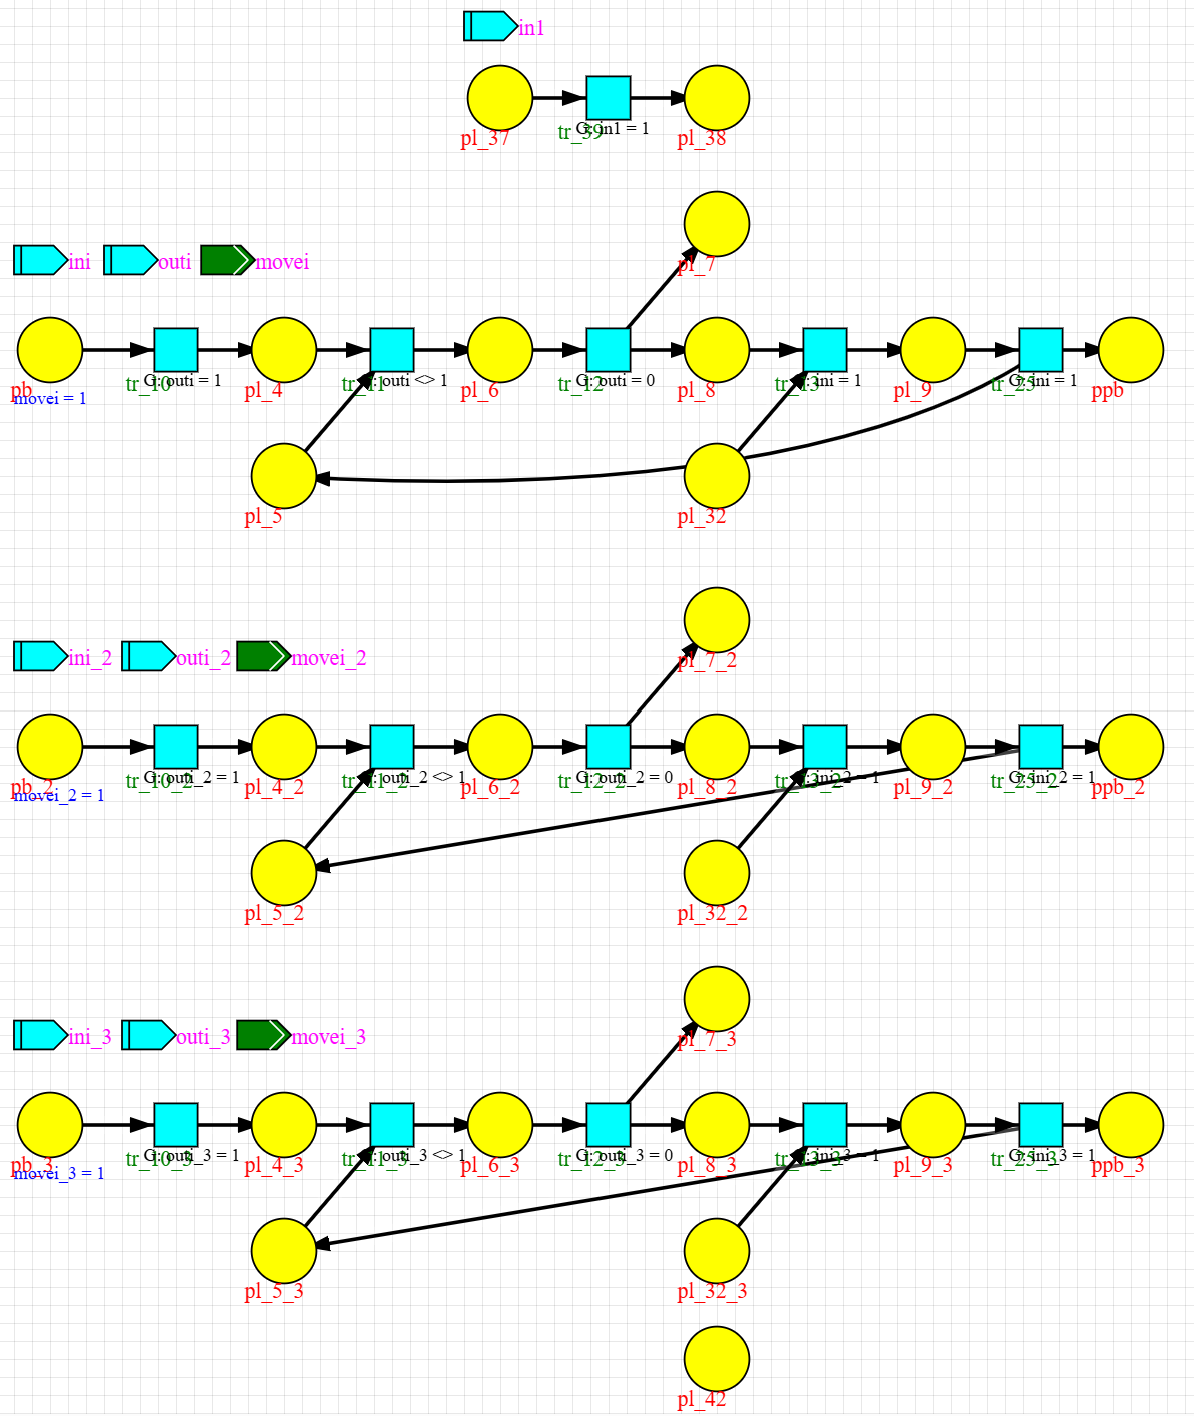
\includegraphics[width=0.8\textwidth]{img/petri_modelo_completo.png}
    \caption{Rede de Petri - Modelo Completo}
    \label{fig:petri_modelo_completo}
\end{figure}

\subsubsection{Rede de Petri - Fusion set}
\begin{figure}[H]
    \centering
    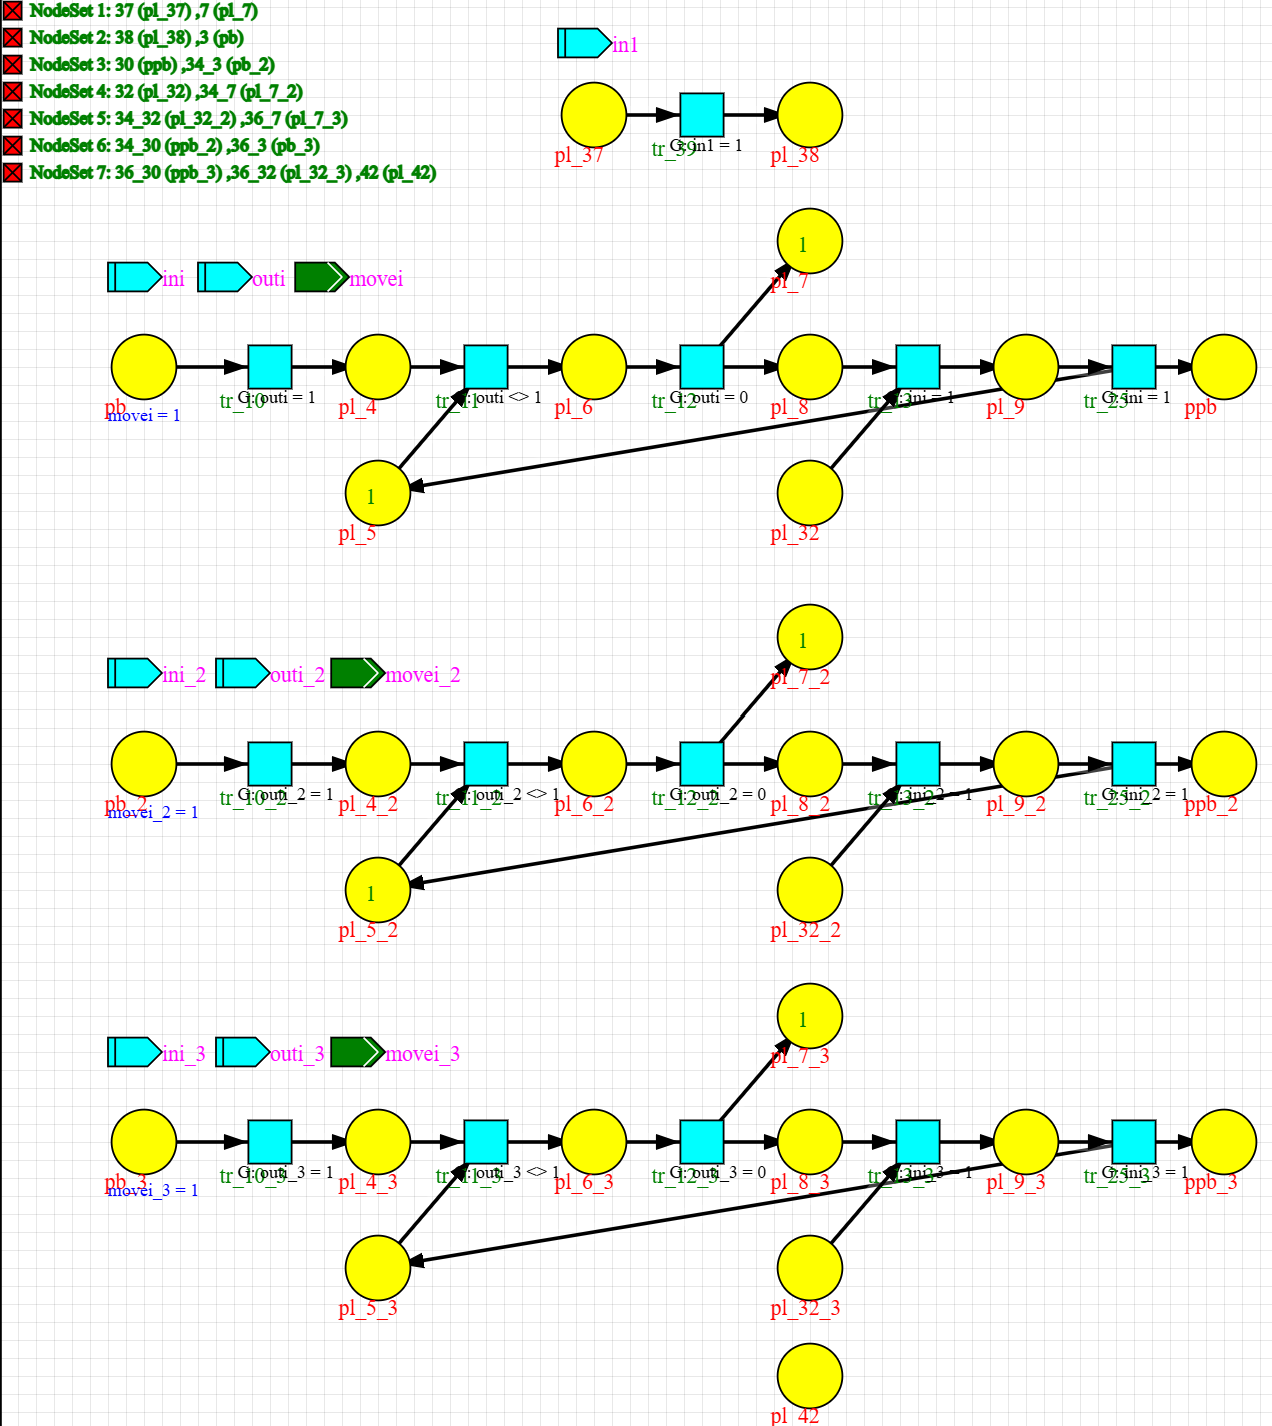
\includegraphics[width=0.8\textwidth]{img/petri_model_merge.png}
    \caption{Rede de Petri - Fusion set}
    \label{fig:petri_fusion_set}
\end{figure}

\subsubsection{Rede de Petri - Node set}
\begin{figure}[H]
    \centering
    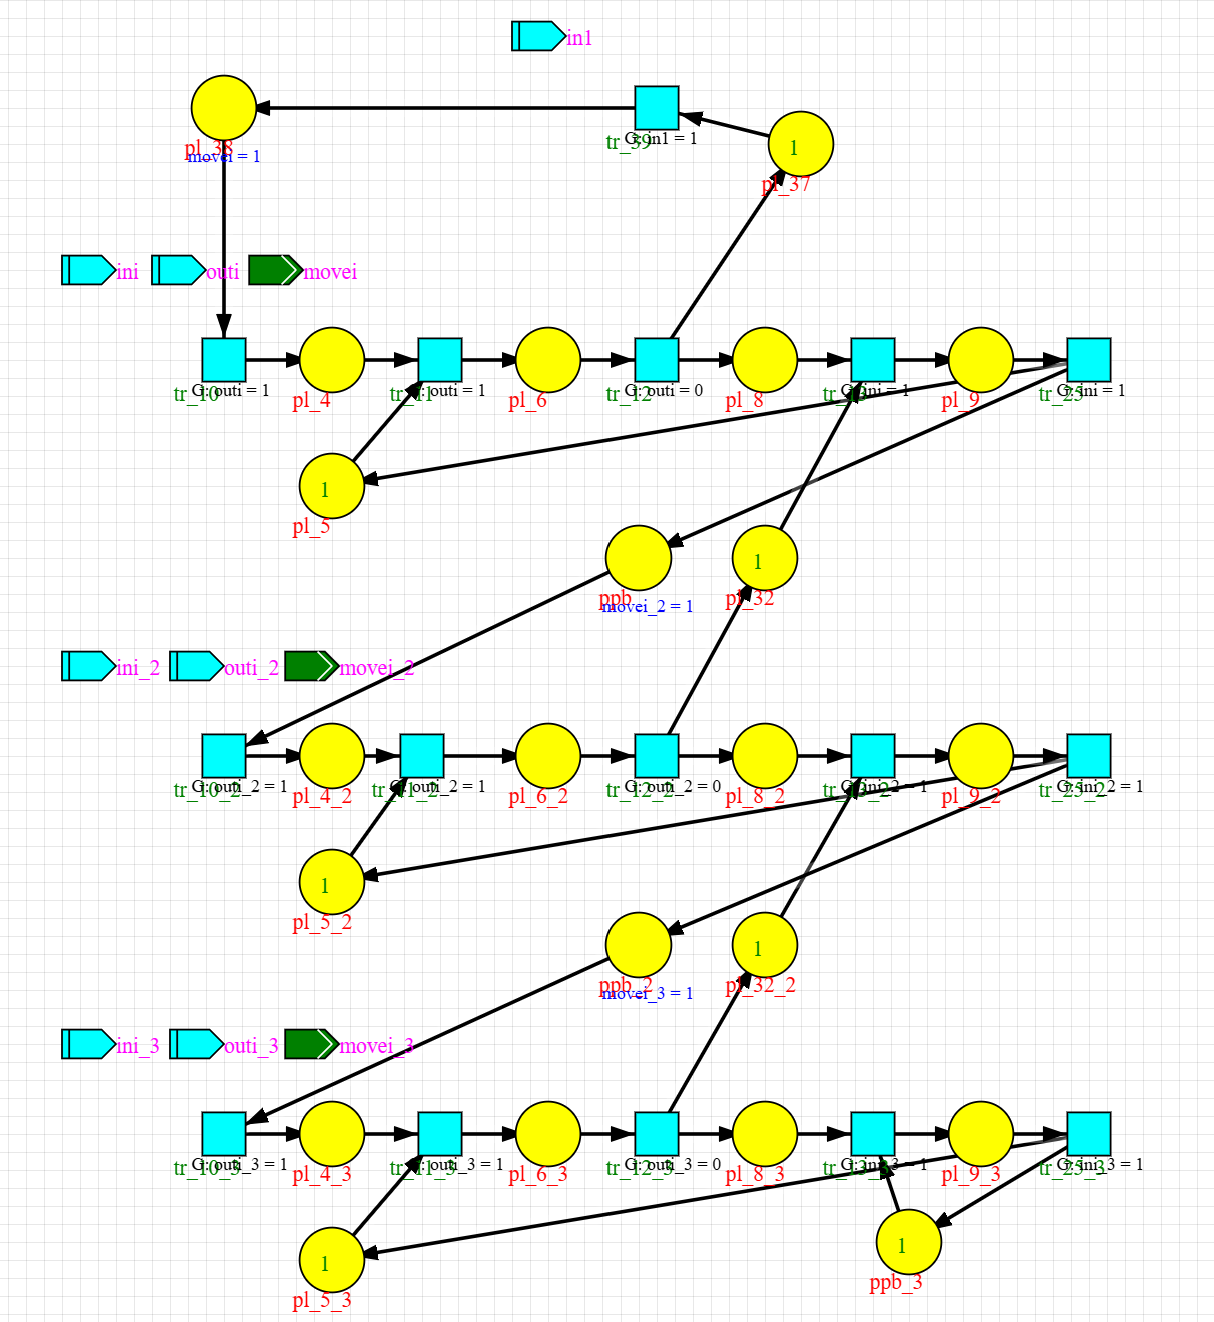
\includegraphics[width=0.8\textwidth]{img/petri_node_set.png}
    \caption{Rede de Petri - Node set}
    \label{fig:petri_node_set}
\end{figure}

\subsection{Simulação e Análise}

\subsubsection{Simulação com token-player}

\subsubsection{Simulação temporal}

\subsubsection{Geração e análise do espaço de estados}

\clearpage

\section{Implementação em FPGA}

\subsection{Geração do código VHDL}

\subsection{Deployment na FPGA}

\subsection{Configuração de entradas/saídas}

\subsection{Testes experimentais}

\subsection{Comparação com resultados de simulação}
\clearpage

\section{Implementação em Arduino}

\subsection{Geração do código C}
\subsection{Deployment no Arduino}
\subsection{Configuração do ambiente}
\subsection{Testes}
\subsection{Comparação com simulação e implementação FPGA}

\clearpage

\section{Controlador Distribuído em regime Síncrono}

\subsection{Identificação do conjunto de corte (cutting set)}

\subsection{Decomposição usando SPLIT}

\subsection{Modelo com canais síncronos}

\subsection{Simulação e validação}

\subsection{Modelo com canais assíncronos}

\subsection{Simulação e Análise}
%Simulação com token-player
%Simulação temporal
%Geração e análise do espaço de estados

\subsection{Decomposição GALS - três controladores separados}

\clearpage

\section{Implementação em FPGA - Distribuição Síncrona}

\subsection{Geração do código VHDL}

\subsection{Interconexão dos componentes}
%Implementação do módulo de atraso pseudo-aleatório
%LFSR - conceito e implementação
%Integração dos atrasos nas comunicações

\subsection{Deployment na FPGA}

\subsection{Testes e análise de resultados}

\clearpage

\section{Buffers de Capacidade Finita}

\subsection{Modificação do modelo para múltiplas peças (máximo 3)}

\subsection{Interconexão dos componentes}

\subsection{Módulo de visualização do número de objetos}

\subsection{Simulação e validação}

\subsection{Implementação centralizada em FPGA}

\subsection{Análise de resultados}


\clearpage

\section{Distribuído com Buffers (Síncrono)}

\subsection{Aplicação síncrona ao buffer de capacidade finita}

\subsection{Decomposição e implementação distribuída}

\subsection{Execução síncrona global}

\subsection{Testes e análise}



\clearpage

\section{Distribuído com Buffers (Assíncrono)}

\subsection{Aplicação assíncrona ao buffer de capacidade finita}

\subsection{Comunicações não-instantâneas com buffers}

\subsection{Deployment e testes}

\subsection{Análise comparativa}


\clearpage

\section{Comparação de abordagens}

\subsection{Centralizado vs Distribuído}

\subsection{Síncrono vs Assíncrono}

\subsection{Impacto dos atrasos de comunicação} 

\subsection{Vantagens e desvantagens de cada abordagem}

\subsection{Análise de escalabilidade}  
\clearpage

\section{Conclusões}

\subsection{Resultados alcançados}
\subsection{Dificuldades encontradas e soluções adotadas}
\clearpage

%==============================================================================
% PÓS-TEXTUAIS
%==============================================================================
% --- Referências bibliográficas ---
\nocite{*}
\bibliographystyle{unsrtnat}  % Estilo de bibliografia numérico
\bibliography{bibliography}
\clearpage  % Garante que o apêndice comece em uma nova página

% --- Apêndice ---
\appendix
% \input{apendix/gnuradiopy}  % Descomente se tiver conteúdo no apêndice

\end{document}